167. \begin{figure}[ht!]
\center{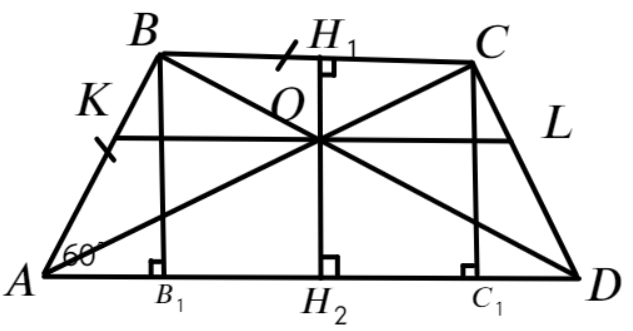
\includegraphics[scale=0.35]{g8-167.png}}
\end{figure}\\
а) Опустим высоты $BB_1$ и $CC_1,$ тогда $AB_1=AB\cos(60^\circ)=6\cdot\cfrac{1}{2}=3,\ B_1C_1=BC=6,\ C_1D=18-3-6=9,\ CC_1=BB_1=AB\sin(60^\circ)=6\cdot\cfrac{\sqrt{3}}{2}=3\sqrt{3},\ CD=\sqrt{27+81}=6\sqrt{3}.$\\
б) В треугольнике $C_1CD$ гипотенуза $CD$ в 2 раза больше катета $CC_1,$ значит $\angle D=30^\circ.$ Также $\angle B=180^\circ-60^\circ=120^\circ,$ а так как треугольник $ABC$ является равнобедренным, $\angle BAC=(180^\circ-120^\circ):2=30^\circ,$ тогда и $\angle CAD=60^\circ-30^\circ=30^\circ.$ Таким образом, $\angle ACD=180^\circ-30^\circ-30^\circ=120^\circ.$\\
в)  Треугольники $BOC$ и $AOD$ подобны по двум углам (вертикальным и накрест лежащим), значит их высоты относятся с тем же коэффициентом, то есть $\cfrac{OH_2}{OH_1}=\cfrac{AD}{BC}=\cfrac{18}{6}=3.$ Так как $OH_1+OH_2=3\sqrt{3},\ OH_2=\cfrac{3}{4}\cdot3\sqrt{3}=\cfrac{9\sqrt{3}}{4}.$ Тогда $S_{\Delta AOB}=S_{\Delta ABD}-S_{\Delta AOD}=\cfrac{1}{2}\cdot 3\sqrt{3}\cdot 18-\cfrac{1}{2}\cdot \cfrac{9\sqrt{3}}{4}\cdot 18=\cfrac{27\sqrt{3}}{4}.$\\
г) Треугольники $AKO$ с $ABC$ и $DLO$ с $DCB$ подобны по двум углам (общий и соответственный), значит $\cfrac{KO}{BC}=\cfrac{AO}{AC}$ и $\cfrac{OL}{BC}=\cfrac{DO}{DB}.$ Треугольники $AOH_2$ с $ACC_1$ и $ODH_2$ с $DBB_1$ подобны по двум углам (общему и прямому), значит $\cfrac{AO}{AC}=\cfrac{OH_2}{CC_1}=\cfrac{3}{4},\ \cfrac{DO}{DB}=\cfrac{OH_2}{BB_1}=\cfrac{3}{4},$ поэтому $\cfrac{KO}{BC}=\cfrac{OL}{BC}=\cfrac{3}{4},\
KO=OL=\cfrac{3}{4}\cdot6=\cfrac{9}{2},\ KL=KO+OL=9.$\newpage\noindent
